

\documentclass{article}

\usepackage{graphicx}
\usepackage{float}
\usepackage{amsmath}
\usepackage[utf8]{inputenc}

\title{Visión por Computador : Práctica 1}
\author{Eloy Bedia García}

\begin{document}
\maketitle
\newpage

\section*{Ejercicio 1}
\textbf{Usando las funciones de OpenCV, escriba funciones que implementen los siguientes puntos:}
\subsection*{Apartado A}
\textbf{El cálculo de la convolución de una imagen con una máscara Gaussiana 2D.
Mostrar ejemplos con distintos tamaños de máscara y valores de sigma. Valorar
resultados.}

\begin{minipage}{\linewidth}
    \centering
    \begin{minipage}{0.45\linewidth}
        \begin{figure}[H]
			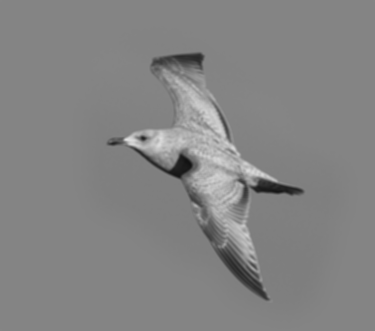
\includegraphics[width=\linewidth]{Ejercicio1a/gaussiana(3,3)3.png} 
            \caption{Kernel Size: 3, $\sigma$: 3}
        \end{figure}
    \end{minipage}
    \hspace{0.05\linewidth}
    \begin{minipage}{0.45\linewidth}
        \begin{figure}[H]
            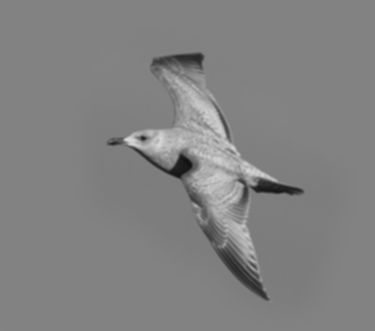
\includegraphics[width=\linewidth]{Ejercicio1a/gaussiana(3,3)4.png}
            \caption{Kernel Size: 3, $\sigma$: 4}
        \end{figure}
    \end{minipage}
    
    \begin{minipage}{0.45\linewidth}
        \begin{figure}[H]
            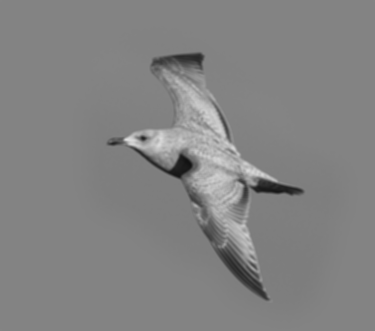
\includegraphics[width=\linewidth]{Ejercicio1a/gaussiana(3,3)5.png}
            \caption{Kernel Size: 3, $\sigma$: 5}
        \end{figure}
    \end{minipage}    
\end{minipage}
\linebreak
Las tres imágenes anteriores, aunque parecen ser la misma, han sido tratadas con distintos filtros gaussianos. En este caso hemos fijado el tamaño del kernel a 3, y hemos variado el valor de $\sigma$. El resultado de los 3 filtros ha sido el mismo ya que el tamño del kernel no es lo suficientemente grande como para poder representar al menos el 95\% de la función gaussiana que define cada filtro.

\begin{minipage}{\linewidth}
    \centering
    \begin{minipage}{0.45\linewidth}
        \begin{figure}[H]
			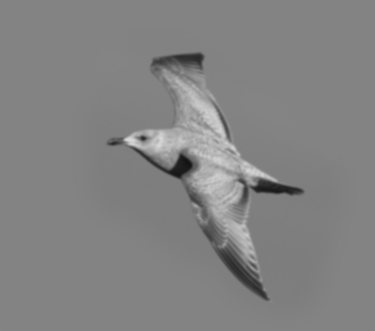
\includegraphics[width=\linewidth]{Ejercicio1a/gaussiana(31,31)1.png} 
            \caption{Kernel Size: 31, $\sigma$: 1}
        \end{figure}
    \end{minipage}
    \hspace{0.05\linewidth}
    \begin{minipage}{0.45\linewidth}
        \begin{figure}[H]
            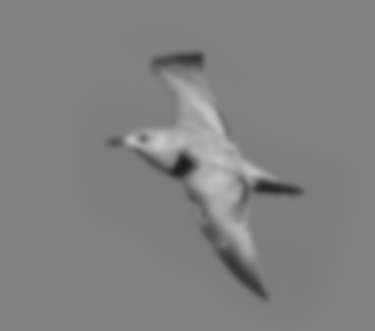
\includegraphics[width=\linewidth]{Ejercicio1a/gaussiana(31,31)3.png}
            \caption{Kernel Size: 31, $\sigma$: 3}
        \end{figure}
    \end{minipage}
    
    \begin{minipage}{0.45\linewidth}
        \begin{figure}[H]
            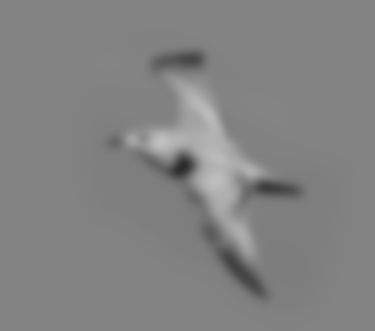
\includegraphics[width=\linewidth]{Ejercicio1a/gaussiana(31,31)5.png}
            \caption{Kernel Size: 31, $\sigma$: 5}
        \end{figure}
    \end{minipage}    
\end{minipage}
\linebreak
En el caso de estas tres imágenes, hemos repetido el experimento escogiendo un tamaño de kernel mas grande. La estadística defiende que el tamaño óptimo de kernel en función de $\sigma$:

\begin{center}
$ksize = 6 \sigma + 1$
\end{center}

En este experimento hemos fijado el tamaño de kernel para el máximo valor de sigma ($\sigma$ = 5). Con esto conseguimos, tal y como hemos dicho antes, representar al menos el 95\% de la función gaussiana.

\subsection*{Apartado B}
\textbf{Usar getDerivKernels para obtener las máscaras 1D que permiten calcular al convolución 2D con máscaras de derivadas. Representar e interpretar dichas máscaras 1D para distintos valores de $\sigma$.}

La función getDerivKernels genera mascaras 1D que permiten calcular la convolución con mascaras 2D (estas mascaras 2D son separables). Tiene 3 parametros:
\begin{itemize}
\item dx $\rightarrow$ nivel de la derivada en X 
\item dy $\rightarrow$ nivel de la derivada en Y
\item ksize $\rightarrow$ el tamaño del kernel
\end{itemize}

La mascara 1D para la primera derivada en X es:
\begin{center}
$$
\begin{pmatrix}
-1 & 0 & 1
\end{pmatrix}
$$
\end{center}

La mascara 1D para la segunda derivada en X es:
\begin{center}
$$
\begin{pmatrix}
1 & -2 & 1
\end{pmatrix}
$$
\end{center}

La mascara 1D para la primera derivada en Y es:
\begin{center}
$$
\begin{pmatrix}
-1 \\
0 \\
1
\end{pmatrix}
$$
\end{center}

La mascara 1D para la segunda derivada en Y es:
\begin{center}
$$
\begin{pmatrix}
1  \\
-2 \\
1
\end{pmatrix}
$$
\end{center}

Podemos observar que la diferencia entre los respectivos niveles de derivación entre X e Y es que las mascaras de X son las transpuestas de Y.
\\

Todas las máscaras cumplen que la sumatoria de sus compoentes resulta 0.



\subsection*{Apartado C}
\textbf{Usar la función Laplacian para el cálculo de la convolución 2D con una máscara de Laplaciana-de-Gaussiana de tamaño variable. Mostrar ejemplos de funcionamiento usando dos tipos de bordes y dos valores de $\sigma$ 1 y 3.}

\begin{minipage}{\linewidth}
    \centering
    \begin{minipage}{0.45\linewidth}
        \begin{figure}[H]
			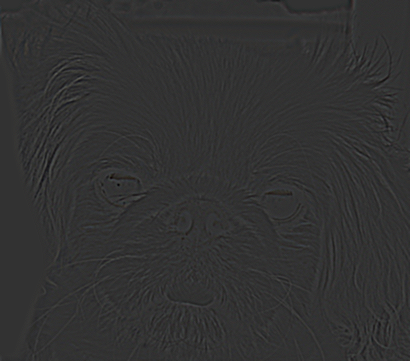
\includegraphics[width=\linewidth]{Ejercicio1c/dog(7,7)1_DEFAULT.png}             			
			\caption{Kernel Size: 7, $\sigma$: 1, Default Border}
        \end{figure}
    \end{minipage}
    \hspace{0.05\linewidth}
    \begin{minipage}{0.45\linewidth}
        \begin{figure}[H]
            
\includegraphics[width=\linewidth]{Ejercicio1c/dog(19,19)3_DEFAULT.png}            
            \caption{Kernel Size: 19, $\sigma$: 3, Default Border}
        \end{figure}
    \end{minipage}
    
    \centering
    \begin{minipage}{0.45\linewidth}
        \begin{figure}[H]
            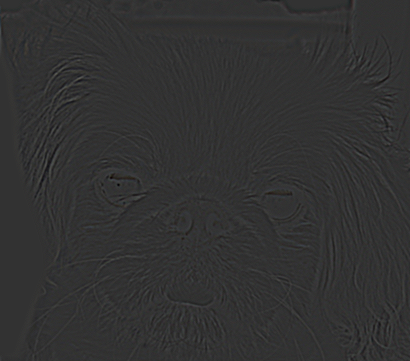
\includegraphics[width=\linewidth]{Ejercicio1c/dog(7,7)1_REFLECT.png}                        
            \caption{Kernel Size: 7, $\sigma$: 1, Reflect Border}
        \end{figure}
    \end{minipage}
    \hspace{0.05\linewidth}
    \begin{minipage}{0.45\linewidth}
        \begin{figure}[H]
            
\includegraphics[width=\linewidth]{Ejercicio1c/dog(19,19)3_REFLECT.png}
            \caption{Kernel Size: 19, $\sigma$: 3, Reflect Border}
        \end{figure}
    \end{minipage}   
\end{minipage}
\linebreak

Para hacer cada una de las imágenes, hemos aplicado un filtro Laplaciano sobre un filtro Gaussiano.
\\

El filtro Laplaciano, resalta los cambios de intensidad en la imagen (aristas), mientras que el Gaussiano, suaviza la imagen para eliminar ruidos.
\\

En primer lugar, vamos a observar las diferencias entre las imágenes debido al valor de $\sigma$ escogido (notese que el el tamaño del kernel es el óptimo para cada $\sigma$).
\\

A mayor sigma, más se suaviza la imagen, por tanto la diferencia de intensidades entre los pixeles van decreciendo. Es por este motivo por lo que la imagen calculada para $\sigma$ igual a 1, tiene las aristas más marcadas que la imagen calculada con $\sigma$ igual a 3.
\\

\newpage
\section*{Ejercicio 2}
\textbf{Implementar apoyandose en las funciones getDerivKernels, getGaussianKernel, pyrUp(), pyrDown(), escribir funciones los siguientes}

\subsection*{Apartado A}
\textbf{El calculo de la convolución 2D con una máscara separable de tamaño variable. Usar bordes reflejados. Mostrar resultados}
\\

La máscara que se ha aplicado en esta imagen es una derivada de primer orden en el eje de las X y una derivada de segundo orden en el eje de las Y.
\linebreak
Esto hace que en el eje de las X resalte las aristas 

\begin{minipage}{\linewidth}
    \centering
    \begin{minipage}{0.45\linewidth}
        \begin{figure}[H]
			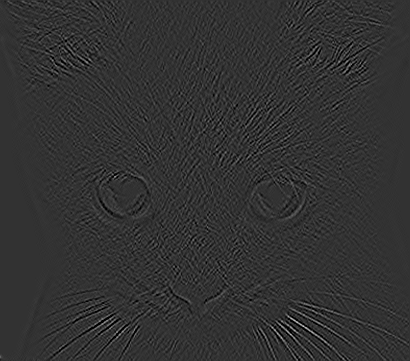
\includegraphics[width=\linewidth]{Ejercicio2a/cat(3,3)_REFLECT.png}             
			\caption{Kernel Size: 3,  Reflect Border}
        \end{figure}
    \end{minipage}   
\end{minipage}

\subsection*{Apartado B}
\textbf{El cálculo de la convolución 2D con una máscara 2D de 1a derivada de tamaño variable. Mostrar ejemplos de funcionamiento usando bordes a cero.}

Una máscara de primera derivada resaltan las aristas de una imagen. Poniendo el ejemplo con mascaras 1D, esto lo consigue dandole al pixel \textit{i} el valor de la diferencia entre sus adyacentes, por tanto si el valor de los pixeles son muy parecidos el pixel apenas responderá (pixel negro), y si los pixeles son extremandamente diferentes el pixel será parte de una arista(pixel blanco)

\begin{minipage}{\linewidth}
    \centering
    \begin{minipage}{0.45\linewidth}
        \begin{figure}[H]
			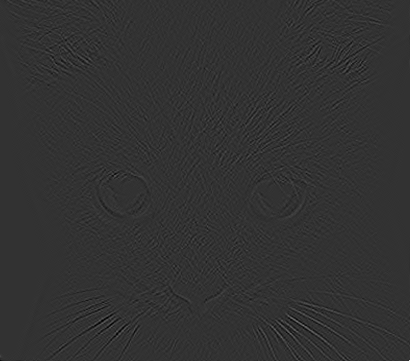
\includegraphics[width=\linewidth]{Ejercicio2b/cat(3,1,1)_DEFAULT.png}             
			\caption{Kernel Size: 3, dx = 1, dx = 1,  Default Border}
        \end{figure}
    \end{minipage}   
\end{minipage}

\subsection*{Apartado C}
\textbf{El cálculo de la convolución 2D con una máscara 2D de 2ª derivada de tamaño variable.}


\begin{minipage}{\linewidth}
    \centering
    \begin{minipage}{0.45\linewidth}
        \begin{figure}[H]
			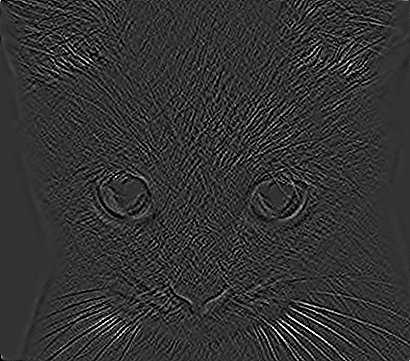
\includegraphics[width=\linewidth]{Ejercicio2c/cat(3,2,2)_DEFAULT.png}             			
			\caption{Kernel Size: 3, dx = 2, dy = 2,  Default Border}
        \end{figure}
    \end{minipage}   
\end{minipage}

\subsection*{Apartado D}
\textbf{Una función que genere una representación en pirámide Gaussiana de 4 niveles de una imagen. Mostrar ejemplos de funcionamiento usando bordes}

La pirámide gaussiana de \textit{n} niveles es un conjunto de tamaño \textit{n} de imágenes formado por la imagen original y \textit{n-1} "reescalados".

Cada uno de los "reescalados" se hace de la siguiente forma: partiendo de la imagen del nivel anterior, se eliminan las filas y columnas pares (o impares) y a continuación se suaviza la imagen (gaussiana).

Si no aplicaramos el suavizado, intruduciríamos ruido, ya que estamos eliminando la mitad de las columnas y filas de la imagen. Aplicando el suavizado, conseguimos minimizar el ruido minimizando la diferencia (debido a la perdida de información de intensidades de los pixeles adyacentes.

\begin{figure}[H]
\centering
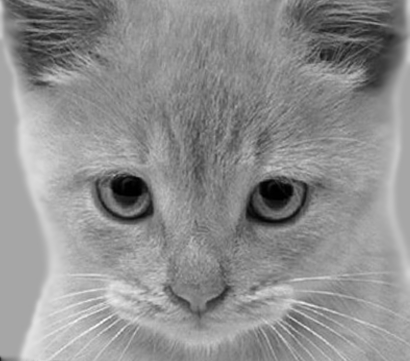
\includegraphics[scale=1]{Ejercicio2d/cat0.png}
\caption{Original}
\end{figure}

\begin{figure}[H]
\centering
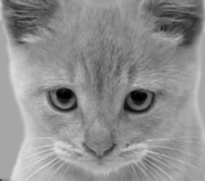
\includegraphics[scale=1]{Ejercicio2d/cat1.png}
\caption{Level 1}
\end{figure}

\begin{figure}[H]
\centering
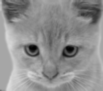
\includegraphics[scale=1]{Ejercicio2d/cat2.png}
\caption{Level 2}
\end{figure}

\begin{figure}[H]
\centering
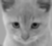
\includegraphics[scale=1]{Ejercicio2d/cat3.png}
\caption{Level 3}
\end{figure}

\begin{figure}[H]
\centering
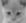
\includegraphics[scale=1]{Ejercicio2d/cat4.png}
\caption{Level 4}
\end{figure}



\subsection*{Apartado E}
\textbf{Una función que genere una representación en pirámide Laplaciana de 4 niveles de una imagen. Mostrar ejemplos de funcionamiento usando bordes.}



\begin{figure}[H]
\centering
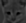
\includegraphics[scale=1]{Ejercicio2e/cat0.png}
\caption{Level 0}
\end{figure}

\begin{figure}[H]
\centering
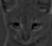
\includegraphics[scale=1]{Ejercicio2e/cat1.png}
\caption{Level 1}
\end{figure}

\begin{figure}[H]
\centering
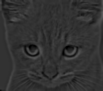
\includegraphics[scale=1]{Ejercicio2e/cat2.png}
\caption{Level 2}
\end{figure}

\begin{figure}[H]
\centering
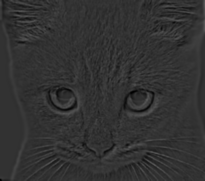
\includegraphics[scale=1]{Ejercicio2e/cat3.png}
\caption{Level 3}
\end{figure}

\begin{figure}[H]
\centering
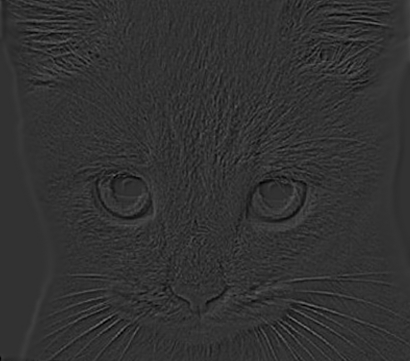
\includegraphics[scale=1]{Ejercicio2e/cat4.png}
\caption{Level 3}
\end{figure}



\section*{Ejercicio 3}
Mezclando adecuadamente una parte de las frecuencias altas de una imagen con una parte de las frecuencias bajas de otra imagen, obtenemos una imagen híbrida que admite distintas interpretaciones a distintas distancias..
Para seleccionar la parte de frecuencias altas y bajas que nos quedamos de cada una de las imágenes usaremos el parámetro sigma del nucleo/máscara de alisamiento gaussiano que usaremos. A mayor valor de sigma mayor eliminación de altas frecuencias en la imagen convolucionada. Para una buena implementación elegir dicho valor de forma separada para cada una de las dos imágenes. Recordar que las máscaras 1D siempre deben tener de longitud un número impar.
Implementar una función que genere las imágenes de baja y alta frecuencia a partir de las parejas de imágenes. El valor de sigma más adecuado para cada pareja habrá que encontrarlo por experimentación
\subsubsection{Apartado A} Escribir una función que muestre las tres imágenes ( alta, baja e híbrida) en una misma ventana. (Recordar que las imágenes después de una convolución contienen número flotantes que pueden ser positivos y negativos)
\subsubsection{Apartado B} Realizar la composición con al menos 3 de las parejas de
imágenes
\\

Los valores de $\sigma$ han sido obtenidos mediante ensayo-error

\begin{minipage}{\linewidth}
    \centering
    \begin{minipage}{0.45\linewidth}
        \begin{figure}[H]
			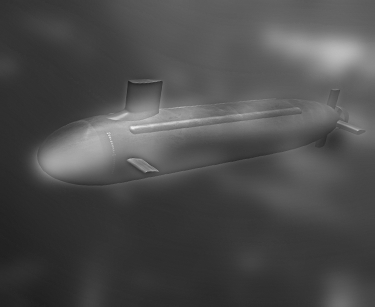
\includegraphics[width=\linewidth]{Ejercicio3/hybrid1.png}          
			\caption{Fish ($\sigma$ = 8) + Submarine ($\sigma$ = 3)}
        \end{figure}
    \end{minipage}
    \hspace{0.05\linewidth}
    \begin{minipage}{0.45\linewidth}
        \begin{figure}[H]
			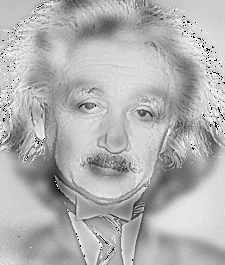
\includegraphics[width=\linewidth]{Ejercicio3/hybrid2.png}          
			\caption{Einstein ($\sigma$ = 2) + Marilyn ($\sigma$ = 4)}
		\end{figure}
    \end{minipage}
    
    \centering
    \begin{minipage}{0.45\linewidth}
        \begin{figure}[H]
            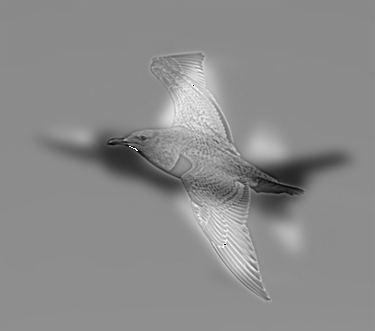
\includegraphics[width=\linewidth]{Ejercicio3/hybrid3.png}          
			\caption{Plane ($\sigma$ = 2) + Bird ($\sigma$ = 6)}
        \end{figure}
    \end{minipage}
    \hspace{0.05\linewidth}
    \begin{minipage}{0.45\linewidth}
        \begin{figure}[H]
            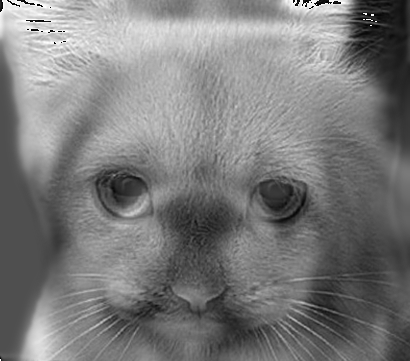
\includegraphics[width=\linewidth]{Ejercicio3/hybrid4.png}          
			\caption{Dog ($\sigma$ = 5) + Cat ($\sigma$ = 3)}
        \end{figure}
    \end{minipage}   
    
     \begin{minipage}{0.45\linewidth}
        \begin{figure}[H]
            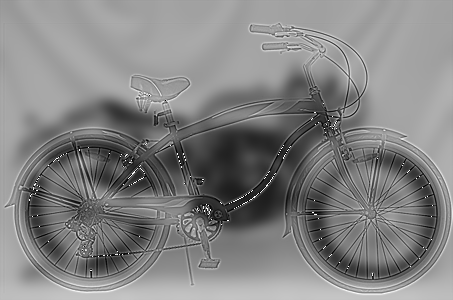
\includegraphics[width=\linewidth]{Ejercicio3/hybrid5.png}          
			\caption{Motorcycle ($\sigma$ = 1) + Bicycle ($\sigma$ = 6)}
        \end{figure}
    \end{minipage}
\end{minipage}


\end{document}